\section{Data Description}

 {
  \begin{figure}[b!]
      \centering
      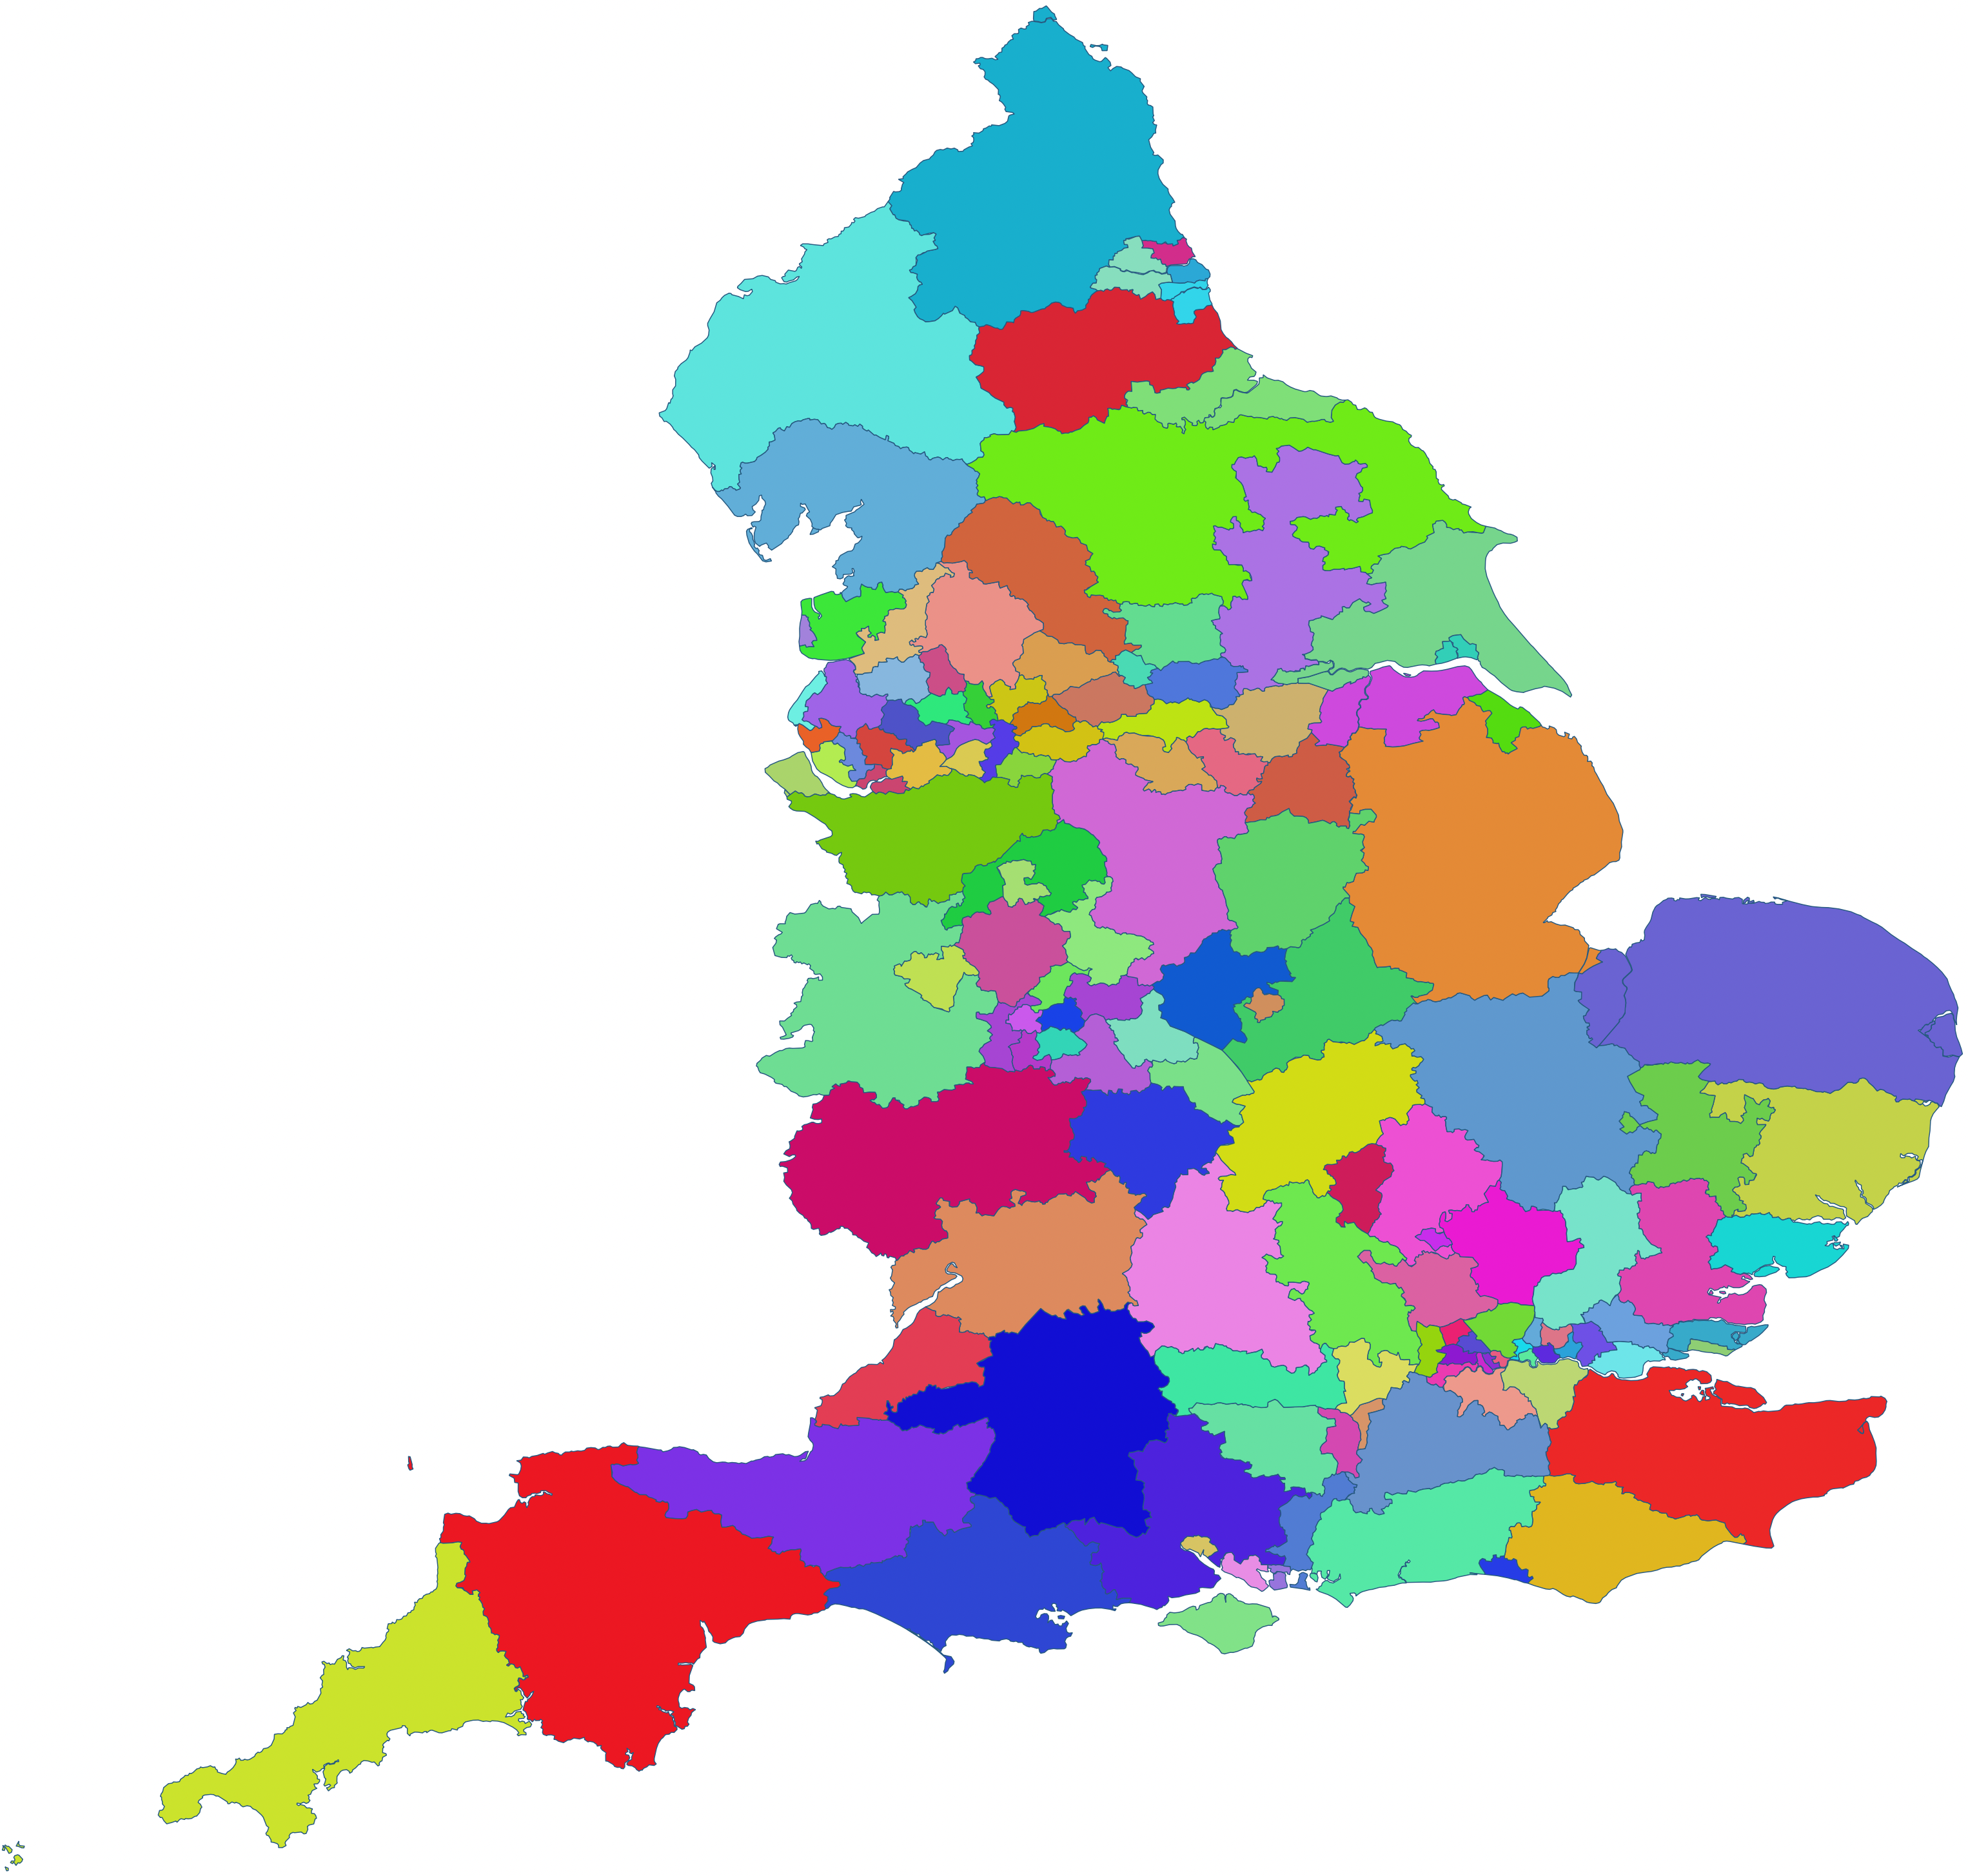
\includegraphics[width=0.6\columnwidth]{figure/ccg.png}
      \caption{A map of 135 CCGs in England as of 2020, obtained from the Open Geography Portalx \cite{opengeographyportalxOpen} with EPSG:4326 (WGS84 - World Geodetic System) as the Coordinate Reference System (CRS).}
      \label{fig:ccg}
  \end{figure}
 }

Obtaining the heterogenous data can be challenging, especially when an EHR dataset is involved, because the data comes from multiple sources \cite{wang2021EHR}. The first step is to obtain both geospatial boundaries and EHR data. The second step is to pre-process the EHR data to remove empty and erroneous values. The final step is to transform the data into a format that is suitable for cartograms. Geospatial boundaries, or shapefiles, were obtained from the sources described here.

\bobgraph{Choropleth Shapefile:} Clinical Commissioning Groups (CCGs) are the primary administrative and geographic unit of the National Health Service (NHS) in the UK \cite{nhsNHS}. The number of CCGs changes over time due to NHS re-organization. The most up-to-date shapefile is available from the Open Geography Portalx \cite{opengeographyportalxOpen}. We decided to use the CCG shapefile from 2020 at the time of writing (See \Cref{fig:ccg}), due to the absence of public EHR data published based on the latest CCG re-organizations that took place in 2021 and 2022.

\bobgraph{River Shapefiles:} We used OpenStreetMap \cite{openstreetmapRelation} as our data source to obtain shapefiles for River Thames, River Trent, and River Great Ouse in England. These rivers were chosen as they are well-known rivers and pass through regions with dense populations, and provide informative geographical and topological cues. While including smaller rivers is technically feasible it may not increase the legibility of the cartogram.

We first obtain a relation ID by searching for a river, e.g. River Thames, on OpenStreetMap. The relation ID is used to construct a query (See Listing~\ref{overpass}) which enables the user to download the entire river shapefile using Overpass Turbo \cite{overpassturboOverpass}.

\begin{lstlisting}[float=tp,caption={The query that downloads the shapefile of River Thames from OpenStreetMap via the Overpass Turbo API.}, label={overpass},captionpos=b]
    relation(2263653);>>;
    // River Great Ouse: 2798097
    // River Trent: 2863468
    out skel;
\end{lstlisting}

After acquiring the shapefiles, we used QGIS \cite{qgisWelcome} to manually adjust projections, and convert them into GeoJSON files. Finally, mapshaper \cite{blochMapshaper} is used to merge and convert the GeoJSON files into a TopoJSON \cite{TopoJSON} file. TopoJSON eliminates redundant coordinates in the data, improving the rendering speed of our implementation. See \Cref{table:pre-processing_result} on page \pageref{table:pre-processing_result} for the pre-processing result. We describe the one-time pre-processing steps in more detail in \Cref{app:pre-processing}.

\bobgraph{EHR Data: }We obtained the Clinical Commissioning Group Outcomes Indicator Set (CCG OIS) from NHS Digital \cite{nhsdigitalClinical}. The OIS is a set of indicators that are used to measure the quality of care and the associated health outcomes in the NHS. Some datasets include:
\begin{itemize}
    \item Under 75 mortality: cardiovascular disease, respiratory disease, liver disease, and cancer
    \item Emergency hospital admission: stroke, alcohol-specific admission and readmission, coronary heart disease, re-admissions within 30 days of discharge, children with lower respiratory tract infections
\end{itemize}

For all datasets, a spreadsheet including the following is provided:

\begin{itemize}
    \item Reporting period: Calendar year of registration
    \item Period of coverage: Start and end date or reporting period
    \item Breakdown: Organization type
    \item ONS code: UK Office for National Statistics CCG code
    \item Level: CCG Code
    \item Level description: CCG Name
    \item Gender
    \item Indicator value: Directly standardized mortality rate
    \item CI lower: lower 95\% confidence interval
    \item CI upper: upper 95\% confidence interval
    \item Denominator: The count of registered patients
    \item Numerator: Number of deaths
\end{itemize}

Each CCG has a unique ONS code, which is used to link the CCG shapefile with the statistical data.